% Copyright 2007 by Till Tantau
%
% This file may be distributed and/or modified
%
% 1. under the LaTeX Project Public License and/or
% 2. under the GNU Public License.
%
% See the file doc/licenses/LICENSE for more details.



\documentclass{beamer}
%\setbeameroption{show notes}

% Setup appearance:

% Standard packages

\usepackage[english]{babel}
\usepackage{times}
\usepackage[T1]{fontenc}
\usepackage{color}
\usepackage[latin1]{inputenc}
\usepackage{chronology}
\usepackage{graphicx}
\usepackage{caption}
\usepackage{subcaption}

\usetheme{Pittsburgh}
\usefonttheme[onlylarge]{structurebold}
\setbeamerfont*{frametitle}{size=\normalsize,series=\bfseries}
\setbeamertemplate{navigation symbols}{}



% Setup TikZ

\usepackage{tikz}
\usetikzlibrary{arrows}
\tikzstyle{block}=[draw opacity=0.7,line width=1.4cm]


% Author, Title, etc.

\title[OpenIdeas] 
{%
	OpenIdeas
}

\author[Amati C., Cardamone S., Leo A., Romano S.]
{
	Ciro Amati\inst{1} \and
  Stefania Cardamone\inst{1} \and
  Amedeo Leo\inst{1} \and
  Simone Romano\inst{1} 
}

\institute[Institute description]
{
  \inst{1}%
		Universit\`a degli Studi di Salerno
  \and
  \vskip-2mm
}

\date[14/12/2015]
{Progetto Web Semantico - Prof.ssa Sabrina Senatore}


% The main document

\begin{document}
\AtBeginSection[]{\begin{frame}{Outline}
 \tableofcontents
    [
        currentsection,
        currentsubsection,
				hideothersubsections
    ]
\end{frame}}
\logo{
\includegraphics[height=1cm]{img/logo.png}}

\begin{frame}
  \titlepage
\end{frame}
\begin{frame}{}
	
	\begin{figure}
		\centering
			
\includegraphics[width=1\textwidth]{img/home.png}
		\label{fig:home}
	\end{figure}
	
		Hai un'idea? Un progetto da realizzare? Con \textbf{OpenIdeas} puoi:
		\begin{enumerate}
			\item Renderla pubblica
			\item Vedere cosa ne pensano gli utenti
			\item Trovare finanziatori
		\end{enumerate}
		
	\begin{figure}
		\centering
			
\includegraphics[width=0.8\textwidth]{img/ideas.png}
		\label{fig:home}
	\end{figure}
\end{frame}

\begin{frame}{Architettura}
	
	\begin{figure}
		\centering
			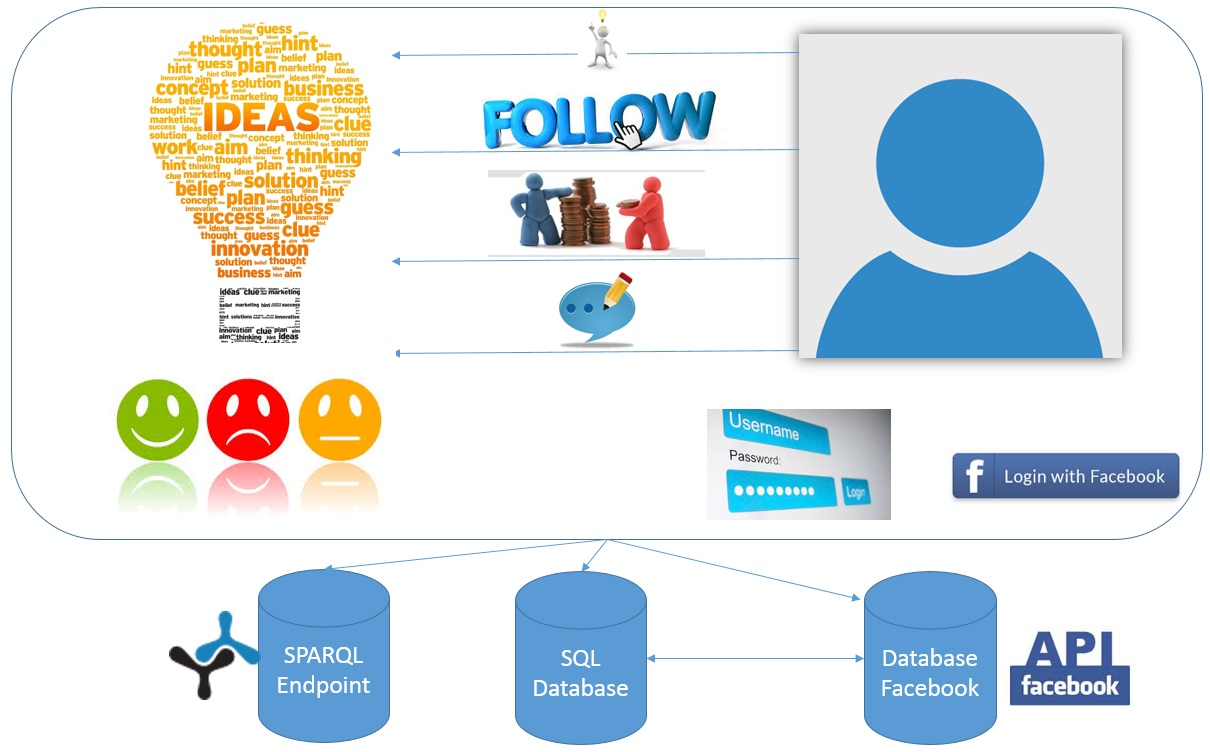
\includegraphics[width=1.00\textwidth]{img/1.jpg}
		\label{fig:architecture}
	\end{figure}
	
\end{frame}

\begin{frame}{Sentiment analysis}
	
	\begin{figure}
		\centering
			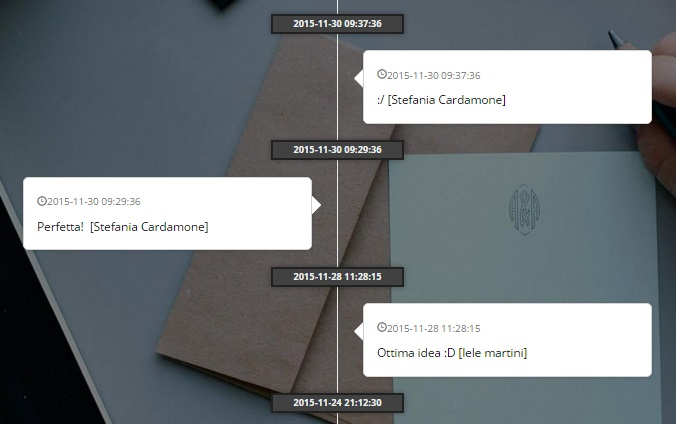
\includegraphics[width=0.5\textwidth]{img/comments.jpg}
		\label{fig:comments}
	\end{figure}
	
	\begin{figure}
		\centering
			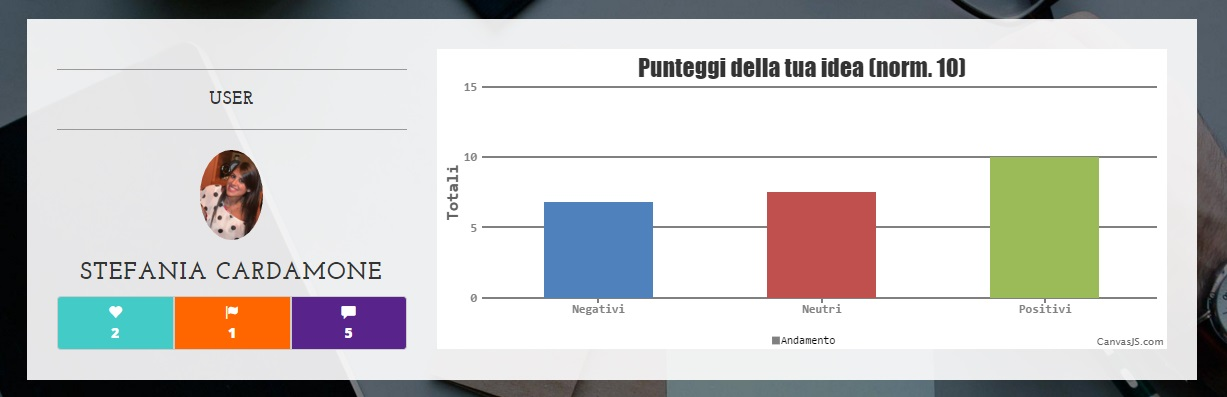
\includegraphics[width=1.00\textwidth]{img/chart.jpg}
		\label{fig:chart}
	\end{figure}
	
	
\end{frame}

\begin{frame}{Linked data}
	
	\begin{figure}
		\centering
			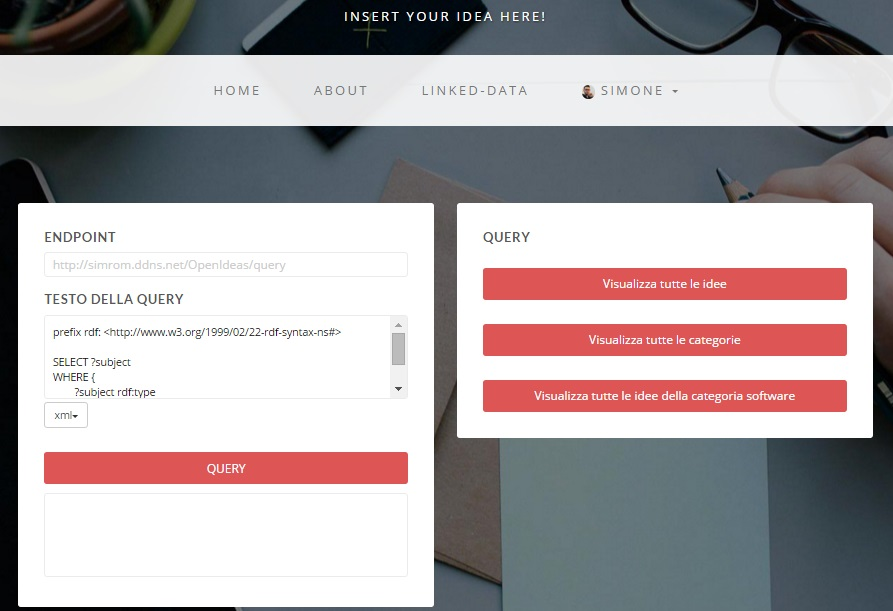
\includegraphics[width=1.00\textwidth]{img/linkedData.jpg}
		\label{fig:linkedData}
	\end{figure}
	
\end{frame}

\begin{frame}{RDFa}
	
	\begin{figure}
		\centering
			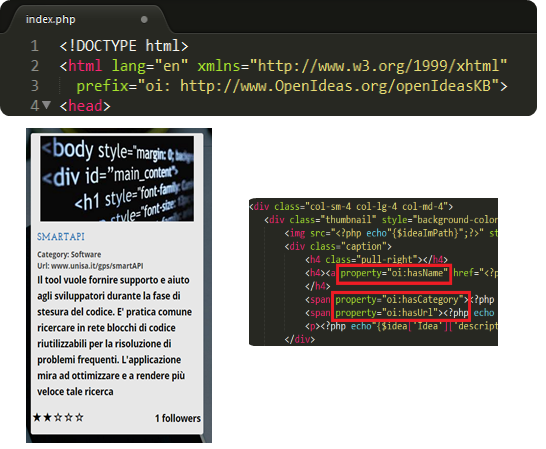
\includegraphics[width=0.8\textwidth]{img/rdfa.png}
		\label{fig:rdfa}
	\end{figure}
	
\end{frame}

\setbeamertemplate{button}{\tikz
  \node[
  inner xsep=10pt,
  draw=structure!80,
  fill=structure!50,
  rounded corners=4pt]  {\Large\insertbuttontext};}

\begin{frame}{Demo}
	
	\begin{center}
		\href{http://localhost/WebSemantico/OpenIdeas/index.php}{\beamergotobutton{Link}}
	\end{center}
\end{frame}

\end{document}

